\aufgabe{Linear models and GAMs}{

In this exercise we are looking at \textit{generalized additive models} or \textit{GAMs}, which are similar to linear models, but instead of terms only containing one feature itself, as in a simple linear model, the terms in GAMs can contain arbitrary smooth functions of one feature.
This means that GAMs can model arbitrary non-linear relationships, but are still additive, meaning every summand only depends on one single feature. Therefore, they do not contain interactions.

Consider the following dataset with 11 observations and two features:

\begin{table}[ht]
	\centering
	\begin{tabular}{crrrrrrrrrrr|r}
		\hline
		& 1 & 2 & 3 & 4 & 5 & 6 & 7 & 8 & 9 & 10 & 11 & $\sum_{i = 1}^n$ \\ 
		\hline
		$y$ & -7.90 & -6.08 & -3.74 & -1.18 & -1.23 & -0.55 & 0.05 & 0.88 & 4.74 & 2.93 & 2.55 & -9.53 \\ 
		$x_1$ & -1.00 & -0.80 & -0.60 & -0.40 & -0.20 & 0.00 & 0.20 & 0.40 & 0.60 & 0.80 & 1.00 & 0.00 \\ 
		$x_2$ & 0.95 & 0.65 & 0.40 & 0.07 & 0.06 & 0.02 & 0.02 & 0.14 & 0.34 & 0.60 & 0.98 & 4.23 \\ 
		\hline
	\end{tabular}
\end{table}

where the last column corresponds to the sum of values of each row.

The following shows the output of an LM ($x_2 \sim x_1$, that means $x_2$ is modeled as a linear function of $x_1$) and a GAM ($x_2 \sim s(x_1)$, that means $x_2$ is modeled as some smooth function of $x_1$):

\begin{center}
	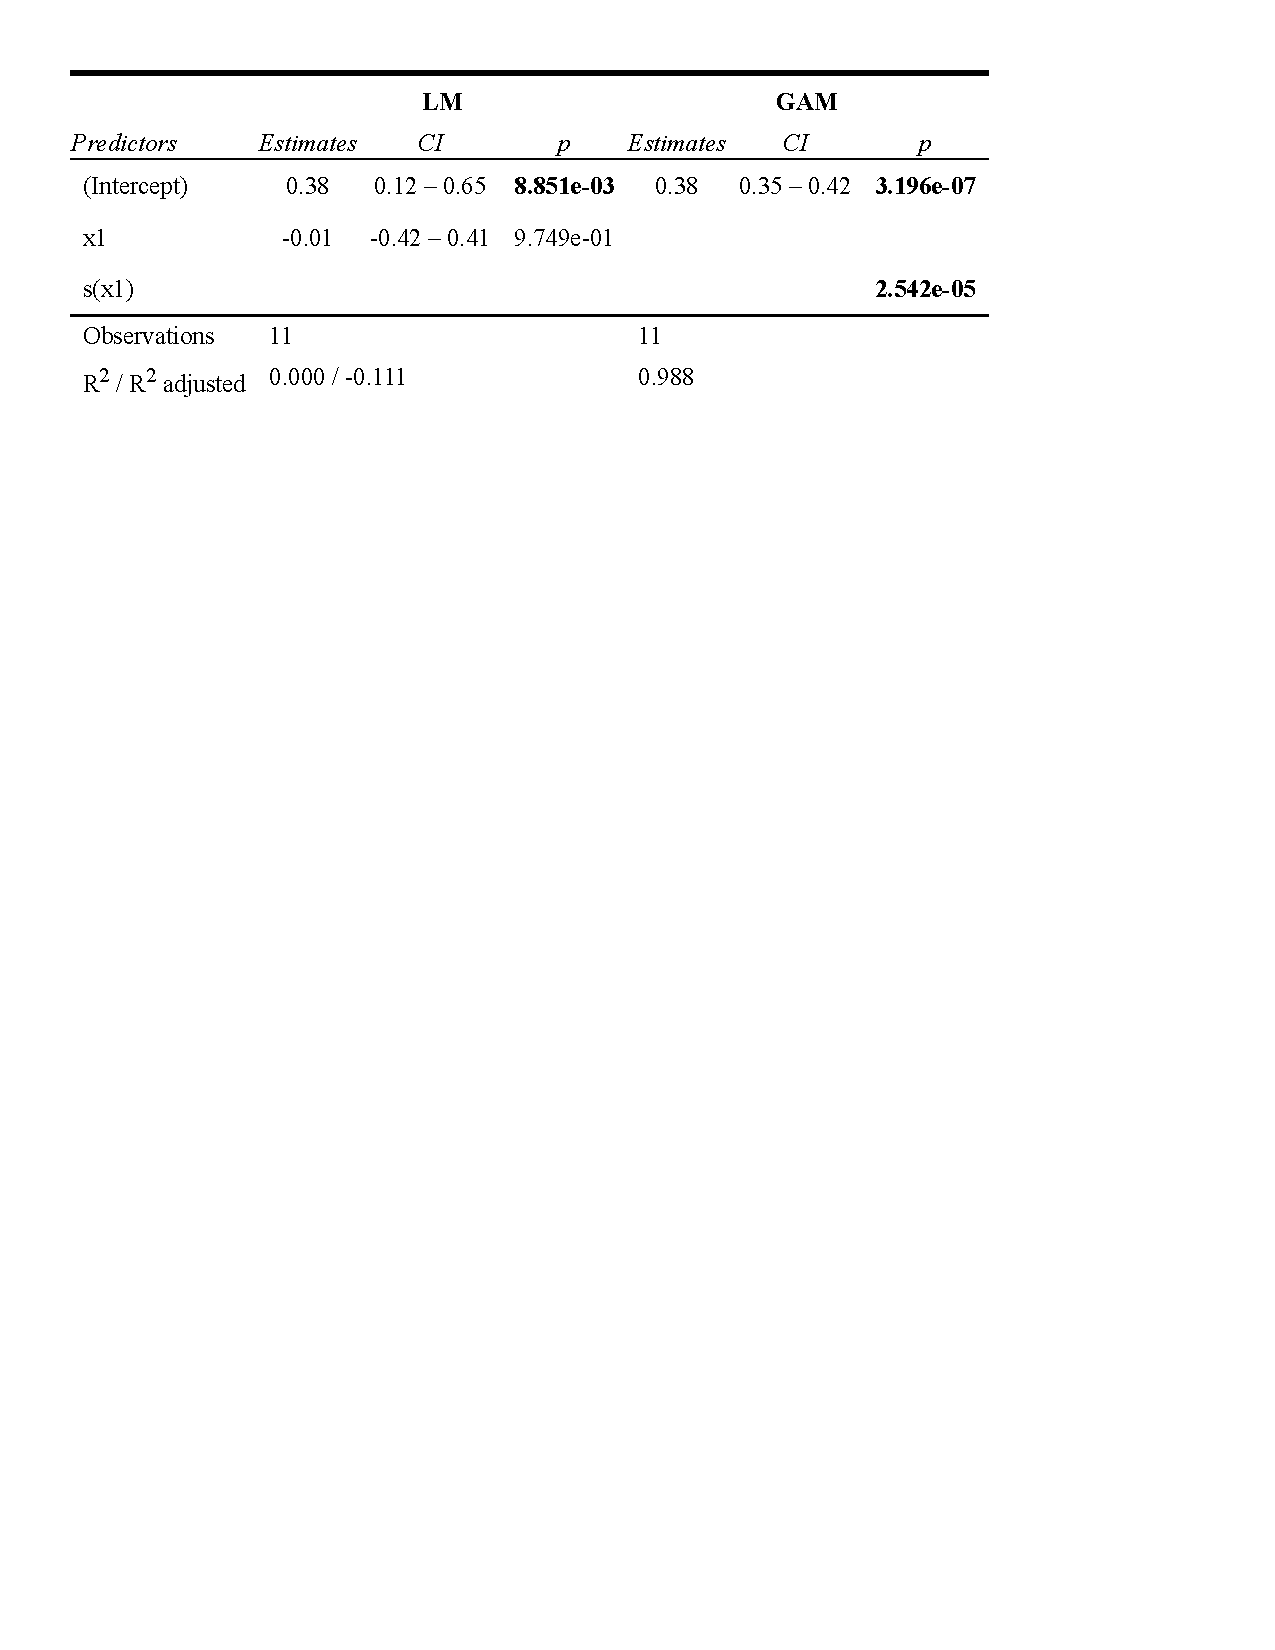
\includegraphics[clip, trim=0.5cm 21cm 5cm 1cm, width=.6\textwidth]{figure/GAM_LM_Output.pdf}
\end{center}

The R$^2$-value for the GAM model is the adjusted one.

\begin{enumerate}[a)]

    \item
    In case you do not know how the adjusted $R^2$ is defined and interpreted, look it up.
    Then interpret the $R^2$ and adjusted $R^2$ values for the two models.
     
	\item
    What conclusions can you draw from the LM model output for the relationship between $x_1$ and $x_2$? 
    
	\item
    Considering the information provided by the GAM model: How can the previous statement about the relationship between $x_1$ and $x_2$ be extended? 
    
\end{enumerate}

}
